\documentclass[12pt]{article}
\usepackage{epsfig}
\usepackage{fullpage}
\title{A First Proof Problem}
\author{Rich Schwartz}

\newtheorem{theorem}{Theorem}[section]
\newtheorem{proposition}[theorem]{Proposition}
\newtheorem{lemma}[theorem]{Lemma}
\newtheorem{sublemma}[theorem]{Sub-Lemma}
\newtheorem{remarks}[theorem]{Remarks}
\newtheorem{corollary}[theorem]{Corollary}
\newtheorem{conjecture}[theorem]{Conjecture}

\def\startproof{{\bf {\medskip}{\noindent}Proof: }}
\def\definition{{\bf {\bigskip}{\noindent}Definition: }}
\def\endproof{$\spadesuit$  \newline}


\def\bp{|\underline{\overline{\times}}|}
\def\A{\mbox{\boldmath{$A$}}}% 
\def\B{\mbox{\boldmath{$B$}}}% 
\def\C{\mbox{\boldmath{$C$}}}% 
\def\D{\mbox{\boldmath{$D$}}}% 
\def\E{\mbox{\boldmath{$E$}}}% 
\def\F{\mbox{\boldmath{$F$}}}% 
\def\G{\mbox{\boldmath{$G$}}}% 
\def\H{\mbox{\boldmath{$H$}}}% 
\def\I{\mbox{\boldmath{$I$}}}% 
\def\J{\mbox{\boldmath{$J$}}}% 
\def\K{\mbox{\boldmath{$K$}}}% 
\def\L{\mbox{\boldmath{$L$}}}% 
\def\M{\mbox{\boldmath{$M$}}}% 
\def\N{\mbox{\boldmath{$N$}}}% 
\def\O{\mbox{\boldmath{$O$}}}% 
\def\P{\mbox{\boldmath{$P$}}}% 
\def\Q{\mbox{\boldmath{$Q$}}}% 
\def\R{\mbox{\boldmath{$R$}}}% 
\def\T{\mbox{\boldmath{$T$}}}% 
\def\U{\mbox{\boldmath{$U$}}}% 
\def\V{\mbox{\boldmath{$V$}}}% 
\def\W{\mbox{\boldmath{$W$}}}% 
\def\X{\mbox{\boldmath{$X$}}}% 
\def\Y{\mbox{\boldmath{$Y$}}}% 
\def\Z{\mbox{\boldmath{$Z$}}}% 
\def\heartsuit{\mbox{\boldmath{$Z$}}}% 



\begin{document}
\noindent
{\bf The Solution:\/}
\newline
\newline
The proof breaks down to two statements.

\begin{enumerate}
\item If $\beta$ is a realized number, then
  $\beta>\sqrt 3$. 
    \item For any $\epsilon>0$ there exists a
  realized number $\beta<\sqrt 3+\epsilon$.
\end{enumerate}

\section{Proof of Statement 1}

{\bf Overview:\/}
We set $G=G_{\beta}$.
The argument is very much like in my paper,
{\it The Optimal Paper Moebius Band\/} (Annals of Math 2025). 
  The connection to
Moebius bands is that the quotient $\Sigma/G$ is a flat
Moebius band, and $f$ induces a map from
$\Sigma/G$ to $\R^3$.
  The main idea is to find two ``crosscutting''
  line segments $(A,B)$ in the strip $\Sigma$,
  having their endpoints in $\partial \Sigma$,
  such that $f(A)$ and $f(B)$ are perpendicular and coplanar line
  segments with disjoint interiors
  that are respectively longer than $A$ and $B$.
  We then compare
  the trapezoid bounded by $A$ and $G(A)$,
  a fundamental domain for the action of $G$,
  with the geometry forced by $f(A)$ and $f(B)$.
 \newline
 \newline
 {\bf Crosscuts:\/}
The $G$-{\it orbit\/} of a subset or a point of the strip
$\Sigma=\R \times [0,1]$
 is the image of that subset or point under
 the action of $G$.  Our second condition on $f$ is
 that $f(p)=f(q)$ if and only if the points $p$ and $q$ are
 in the same $G$-orbit.
 We call our clean triangulation
 $\cal C$ and we call the triangles of the clean triangulation
 ${\cal C\/}$-{\it triangles\/}.   Because $\cal C$ is
  locally finite, the
 ${\cal C\/}$-triangles are
 ordered left to right, with consecutive triangles
 sharing an edge.

 Recall that the {\it distinguished edge\/} of a ${\cal C\/}$-triangle
 is the edge in $\partial \Sigma$.
The {\it distinguished vertex\/} of a ${\cal C\/}$-triangle is
the vertex opposite the distinguished edge.  This is the vertex
in the other boundary component.
Say that a {\it crosscut\/} is a line segment $A \subset \Sigma$ that
joins the distinguished vertex of a ${\cal C\/}$-triangle $\tau$
to a point on the distinguished edge of $\tau$.
The interior of the strip $\Sigma$ is foliated by the (relative) interiors
of the crosscuts.

Given two crosscuts
$A$ and $B$ we write $A \prec B$ is the midpoint of $A$ lies
to the left of the midpoint of $B$. (Both these midpoints lie on the
centerline of $\Sigma$.)   We call the pair
$(A,B)$ {\it admissible\/} if $A \prec B \prec G(A)$.
This condition implies that $A$ and $B$ have
different $G$-orbits.
Note that $(A,B)$ is admissible if and only if
\begin{equation}
  \label{involute}
  I(A,B):=(B,G(A))
\end{equation}
is admissible. The map $I$ is a self-map of the set of admissible
pairs of crosscuts.

\begin{lemma}
  \label{adm}
  If $(A,B)$ is an admissible pair, then
  $f(A)$ and $f(B)$ have disjoint interiors.
\end{lemma}

\startproof
If not, then
there are interior points $p \in A$ and $q \in B$ such
that $f(p)=f(q)$.  But then the $G$-orbit of
${\rm interior\/}(A)$ intersects the $G$-orbit of ${\rm interior\/}(B)$.   Since our
crosscuts have disjoint interiors, this means
that $A$ and $B$ have the same $G$-orbit.
Contradiction.
\endproof

\begin{lemma}
  \label{expand}
  $f$ increases arc length on each crosscut.
\end{lemma}

\startproof
Recall that $f$ is a squeeze map on each triangle $\tau$.
So $\phi:=f|_{\tau}$ is affine, and $\phi$ decreases the length of
the distingished edge of $\tau$ and increases the lengths of
the other edges.
Let $p$ be the distinguished vertex of $\tau$
and let $q$ be any point in the distinguished
edge.  We just need to see that $\phi$ increases the distance from
$p$ to $q$.

Without loss of generality we can translate
the picture so that $p$ and $f(p)$ are the origin respectively
in $\R^2$ and in $\R^3$.   Then $\phi$ is a linear
transformation.  Setting $V'=f(V)$, etc, this
lemma is equivalent to the following.  We have
vectors $V,W,V',W'$ such that
\begin{equation}
  \label{squeeze}
\|V\|<\|V'\|, \hskip 20 pt
\|W\|<\|W'\|, \hskip 20 pt
\|V-W\|>\|V'-W'\|,
\end{equation}
and we want to see that
$\|(1-t)V+tW\|<\|(1-t)V'+tW'\|$
for all $t \in (0,1)$.
This last inequality is true provided that
$V \cdot W < V'\cdot W'$.
Squaring the inequalities in Equation \ref{squeeze},
$$2V \cdot W = \|V\|^2 + \|W\|^2  - \|V-W\|^2<
\|V'\|^2+\|W'\|^2 - \|V'-W'\|^2 = 2V' \cdot W'.$$
So, indeed, $V \cdot W < V' \cdot W'$.
\endproof

\noindent
{\bf The Key Topological Idea:\/}
This proof has the same ideas as Lemma T in my paper.

\begin{lemma}[T]
  $\Sigma$ has a pair $(A,B)$ of admissible crosscuts such that
  $f(A)$ and $f(B)$ are perpendicular and coplanar.
\end{lemma}

\startproof
Let $\cal A$ denote the set of all admissible pairs.
We parametrize the set of crosscuts by $\R$:  Each crosscut is
parametrized by the $X$-coordinate of its midpoint.
With this parametrization,
${\cal A\/} \subset \R^2$ is the interior of the closed infinite strip $\overline{\cal A}$
bounded by the lines $y=x$ and $y=x+\beta$.  We call these
lines respectively
$\partial_0{\cal A}$ and $\partial_1{\cal A\/}$.
The map $I$ from Equation \ref{involute} acts as a glide reflecton on
$\cal A$, namely $I(x,y)=(y,x+\beta)$.

For any subset $X \subset \Sigma$ let $X'=G(X)$.
We direct each crosscut $C$ so that it points upwards.
We orient $f(C)$ so that $f$ is direction preserving on $C$.
Let $\overrightarrow f(C)$ be the vector that points in the
direction of $f(C)$ and has the same length.  Note
that $\overrightarrow f(C')=-\overrightarrow f(C)$.

Let $(A,B)$ be a pair of crosscuts, with midpoints $a$ and $b$
respectively.
Using the dot product and cross
product, define

\begin{equation}
  \label{def}
  g(A,B)=\overrightarrow f(A) \cdot \overrightarrow f(B), \hskip 20 pt
  h(A,B)= (f(a)-f(b)) \cdot (\overrightarrow f(A) \times \overrightarrow f(B)).
\end{equation}
By construction, $g$ and $h$ are continuous functions on
$\overline{\cal A}$.
Furthermore,  if $g(A,B)=0$ then
$A$ and $B$ are perpendicular.  If
$h(A,B)=0$ then $A$ and $B$ are coplanar.
(If $f(A)$ and $f(B)$ are both parallel to the $XY$-plane then
$h(A,B)$ measures the
difference in the $Z$-coordinates of these segments.)
In view of this, it suffices to prove
that $(0,0) \in \Phi({\cal A\/})$, where $\Phi=(g,h)$.

Using  $f(a')=f(a)$ and  $\overrightarrow
f(C')=-\overrightarrow f(C)$
and the symmetries of the dot and cross products, we establish
the {\it oddness property\/}: 
$\Phi \circ I=-\Phi$.  Here is the derivation.
$$g(B,A')=\overrightarrow f(B') \cdot \overrightarrow f(A)
=-\overrightarrow f(B) \cdot \overrightarrow f(A) =-g(A,B).$$
$$h(B,A')= (f(b)-f(a')) \cdot (\overrightarrow f(B') \times
\overrightarrow f(A))=
(f(b)-f(a)) \cdot (\overrightarrow f(A) \times
\overrightarrow f(B))=-h(A,B).$$

Note that $h=0$ on $\partial \cal A$.
Because $\overrightarrow A$ and $\overrightarrow B$ are
parallel on $\partial_0 \cal A$, we have
$g>0$ on $\partial_0 \cal A$.  Likewise $g<0$ on $\partial_1 \cal A$.
Hence $\Phi(\partial_0 {\cal A\/}) \subset X_+$, the positive $X$-axis, $X_+$.
Likewise $\Phi(\partial_1 {\cal A\/}) \subset X_-$, the negative
$X$-axis.

Suppose $(0,0) \not \in \Phi({\cal A\/})$.
If $\gamma \subset \overline{\cal A\/}$ is a segment
with endpoints in the two boundary components of $\cal A$ then
$\Phi(\gamma)$ is a continuous arc that joins a point
in $X_+$ to a point in $X_-$ and misses the origin.
Therefore, $\Phi(\gamma)$ has a well-defined
half-integer winding number $w(\gamma)$ with respect to the origin.
If $\gamma$ is such a segment, then so is
$\gamma^*=I(\gamma)$.
On the one hand, $\gamma^*$ and $\gamma$ are
isotopic relative to
$\partial_0 \cal A$ and $\partial_1 \cal A$ and
$w(\cdot)$ is continuous and half-integer valued.
Hence $w(\gamma)=w(\gamma^*)$.
On the other hand
$\Phi(\gamma^*)=-\Phi(\gamma)$, by the oddness property.
But then $w(\gamma^*)=-w(\gamma)$, a
contradiction. Hence $(0,0) \in \Phi({\cal A\/})$.
\endproof

\noindent
{\bf The Trapezoid:\/}
Let $(A,B)$ be as in Lemma T.
The images $f(A)$ and $f(B)$ are perpendicular
and coplanar and by Lemma \ref{adm} have disjoint interiors.
Either the line
extending $f(A)$ is disjoint from the interior of $f(B)$ or the line
extending $f(B)$ is disjoint from the interior of $f(A)$.
If necessary we replace $(A,B)$ by $I(A,B)$, which
also satisfies Lemma T, to arrange that the line extending
$f(A)$ is disjoint from the interior of $f(B)$.
Pre-composing and post-composing $f$ by isometries we can
arrange, as in Figure 1, that
\begin{itemize}
\item $f(A)$ lies in
the $X$-axis and $f(B)$ is contained in the non-positive
portion of the $Y$-axis.
\item $f$ maps the upper vertex of $A$ to the left vertex of $f(A)$.
\item $f$ maps the top vertex of $B$ to the top vertex of $f(B)$.
\end{itemize}
Let $t \in \R$ be such that $1/t$ is the slope of $A$.
Figure 1 depicts the case when $t>0$, and
$f(A) \cap f(B)=\emptyset$, but
our argument does not need these conditions.

\begin{center}
  \resizebox{!}{1.8in}{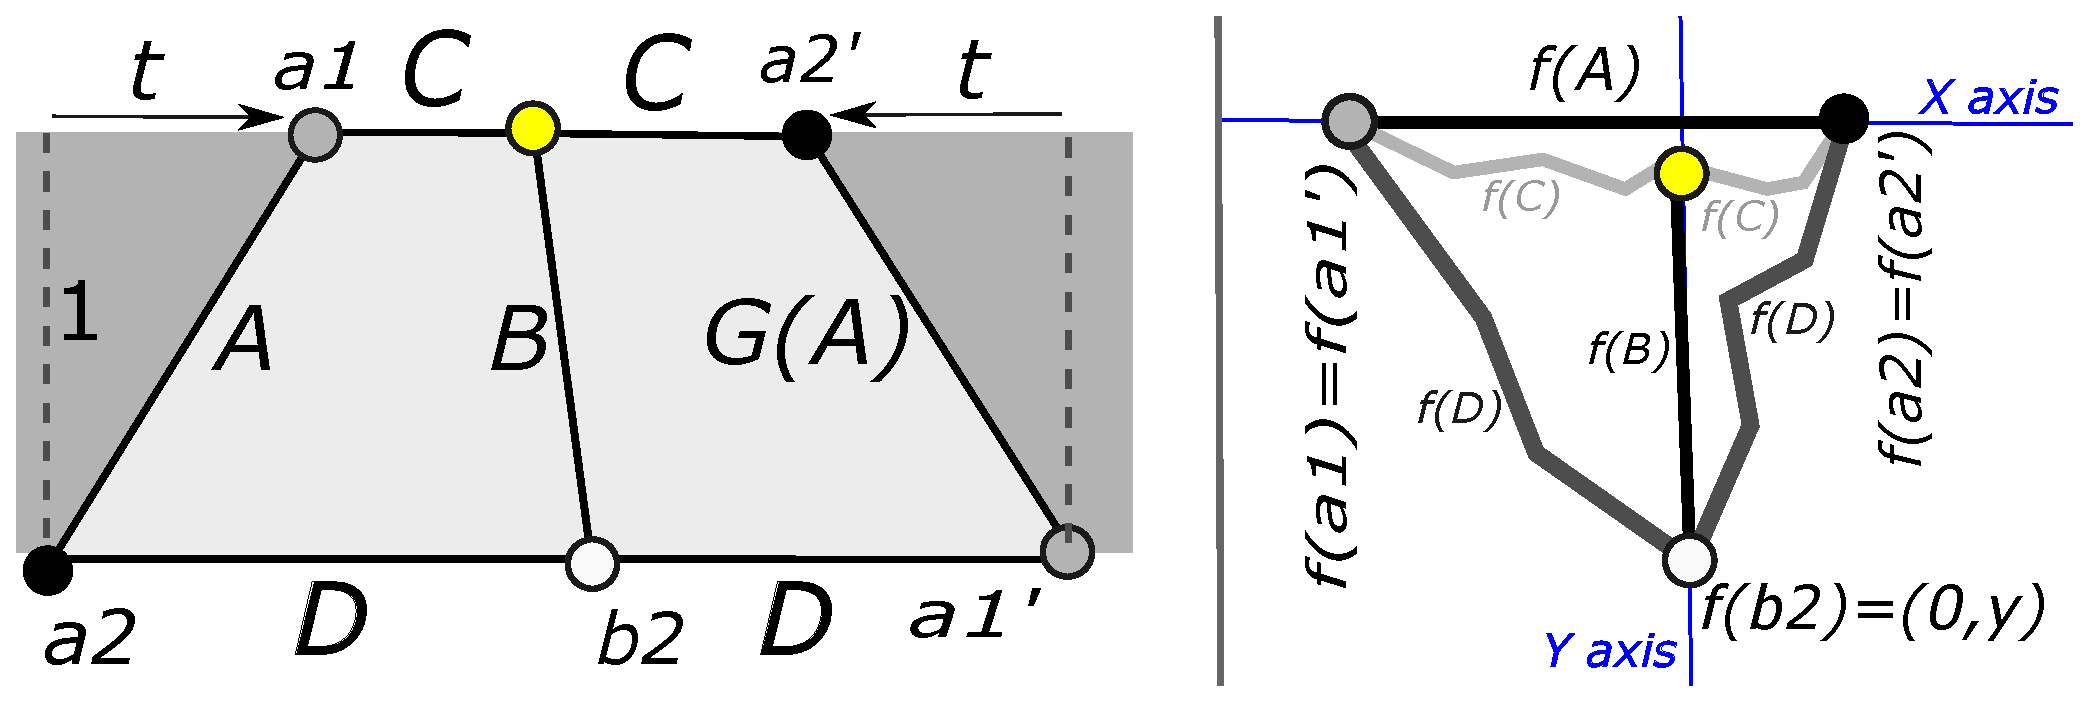
\includegraphics{fig1.eps}}
  \newline {\bf
    Figure 1:\/} The domain is on the left and the range is on the
  right.
  \end{center}


Let $C$ and $D$ be the segments in
$\R \times \{1\}$ and $\R \times \{0\}$,
respectively, connecting the endpoints
of $A$ and $G(A)$. Since $G$ is a glide reflection,
the trapezoid $T$ bounded by $A,C,g(A),D$ is isosceles.
Starting from the bottom left and going clockwise, the
vertices of $T$ are $a_2,a_1,a_2',a_1'$.  We have
$G(a_k)=a_k'$ for $k=1,2$.  In other words,
$G$ identifies the vertices in opposite corners
of $T$. Hence, so does $f$.  Also, $b_2$ denotes
the bottom endpoint of the bend $B$. (The top
endpoint of $B$ is colored yellow in the figure
but has no name.)


Let $\ell$ denote arc-length.
Note that $\ell(A)=\sqrt{1+t^2}$ and $\ell(B) \geq 1$.

\begin{lemma}
  \label{bound}
  $\ell(C)>\sqrt{1+t^2}$ and
   $\ell(D)>\sqrt{5+t^2}$.
\end{lemma}

\startproof
By Lemma \ref{expand}, the map $f$ increases
arc length on each crosscut.  The squeeze map
property implies that $f$ decreases
arc length on $\partial \Sigma$.
Hence $$\ell(f(A))>\ell(A)=\sqrt{1+t^2}, \hskip 15 pt 
              \ell(f(B))>\ell(B) \geq 1, \hskip 15 pt
              \ell(C)>\ell(f(C)), \hskip 15 pt
              \ell(D)>\ell(f(D)).$$
              Since $f(C)$ connects the endpoints of $f(A)$, we have
              $\ell(f(C)) \geq \ell(f(A))$.  All together,
$$\ell(C)>\ell(f(C))  \geq \ell(f(A)) > \ell(A) = \sqrt{1+t^2}.$$

The point $f(b_2)=(0,y)$ separates $f(D)$ into two arcs
$\gamma_1$ and $\gamma_2$.  Let
$\gamma_2^*$ denote the reflection of
$\gamma_2$ in the horizontal line through
$(0,y)$.    We have
$$\ell(D)>\ell(f(D))=\ell(\gamma_1 \cup \gamma_2)=
\ell(\gamma_1 \cup \gamma_2^*) \geq
\sqrt{4y^2+\ell(f(A))^2} \geq \sqrt{5+t^2}.$$
The second equality comes from symmetry.
The final inequalities come from the fact that
$\gamma_1 \cup \gamma_2^*$ connects two
points which are separated horizontally by $\ell(f(A))>\sqrt{1+t^2}$ and vertically by $|2y| \geq
2\ell(f(B))>2$.
\endproof

\noindent
{\bf Endgame:\/}
Given our definition of $t$, Lemma \ref{bound} gives
$$
\beta = \ell(C)+t >  u(t):=\sqrt{1+t^2}+t, $$
\begin{equation}
    \beta = \ell(D)-t >  v(t):=\sqrt{5+t^2}-t.
\end{equation}

Hence $\beta>\max(u(t),v(t))$.
Let $t_0=1/\sqrt 3$.
Note that $u(t_0)=v(t_0)=\sqrt 3$, and
$u$ is an increasing function and
$v$ is a decreasing function.
Hence $\max(u(t),v(t)) \geq \sqrt 3$ for all $t$.
Hence $\beta>\sqrt 3$.
This proves Statement 1.

\section{Proof of Statement 2}

{\bf Overview:\/}
  Let $\epsilon>0$ be given. 
We will produce a realized number $\beta<\sqrt
3+\epsilon$.  We take $\epsilon<1/100$ for convenience.
We build a polyhedral Moebius band $\Omega$ by
stacking three equilateral triangles on top of each other
and connecting them in a cyclic pattern using very thin
rectangles.   We then extract the combinatorial details
and construct our map $f: \Sigma \to \R^3$ having
$\Omega$ as the image.  So, we first describe the
range, then the domain, then the map.
\newline
\newline
{\bf The Range:\/}
Let $\mu=2/\sqrt 3$.
This is the side length of a clean equilateral triangle.
Let
$T_0 \subset \R \times (-\infty,0] \times \{0\}$ be the equilateral triangle,
of side length $\mu + \epsilon^2$, which
has an edge centered at the origin and contained in
the $X$-axis.  Let $\partial_- T_0$, $\partial_+T_0$ and
$\partial_0T_0$ respectively denote the left, right, and
top boundary edge of $T_0$.   See Figure 2 below.

Let $E_0$ denote the segment
$\partial_0 T_0 + (0,\epsilon^3,0)$.
We are translating $\partial_0T_0$ parallel to
itself and slightly off itself.
Figure 2 (left) shows $T_0$ and $E_0$ fairly
accurately.  Here we are looking down on $\R^2 \times \{0\}$.

Define $T_{\pm} = T_0 \pm (0,0,\epsilon^3)$.
These two triangles lie in horizontal planes just above and below
$T_0$.  We label the edges of $T_{\pm}$ so that
$\partial_j T_{\pm}$ is parallel to $\partial_j T_0$.
Here $j \in \{0,+,-\}$.

We now define $3$ sets, $R_+$, $R_-$, and $R_0$.  We call these {\it connectors\/}.
\begin{itemize}
  \item $R_{\pm}$ is a thin rectangle, the convex hull of
    $\partial_{\pm} T_0 \cup \partial_{\pm} T_{\pm}$.   The long
    sides of $R_{\pm}$ have length $\mu+\epsilon^2$ and the short
    sides have length $\epsilon^3$.
  \item $R_0=S_+ \cup S_-$ is the union of two rectangles.
    Here $S_{\pm}$ is the    convex
    hull of $\partial_0 T_{\pm} \cup E_0$.
    The long sides of $S_{\pm}$ have length $\mu+\epsilon^2$ and the short
    sides have length less than $2 \epsilon^3$.
  \end{itemize}

  Note that $R_{\pm}$ connects $\partial_{\pm} T_0$ to $\partial_{\pm}
  T_{\pm}$.  Likewise,
    $R_0$ connects $\partial_0 T_-$ to $\partial_0 T_+$ while remaining
  disjoint from $T_0$.  We used $E_0$ to slightly bend $R_0$ away from
  $T_0$.   Define
    \begin{equation}
    \label{OM}
    \Omega = S_- \cup T_- \cup R_- \cup T_0 \cup R_+ \cup T_+ \cup
    S_+.
  \end{equation}
  Figure 2 (right) shows this union schematically.


\begin{center}
  \resizebox{!}{1.7in}{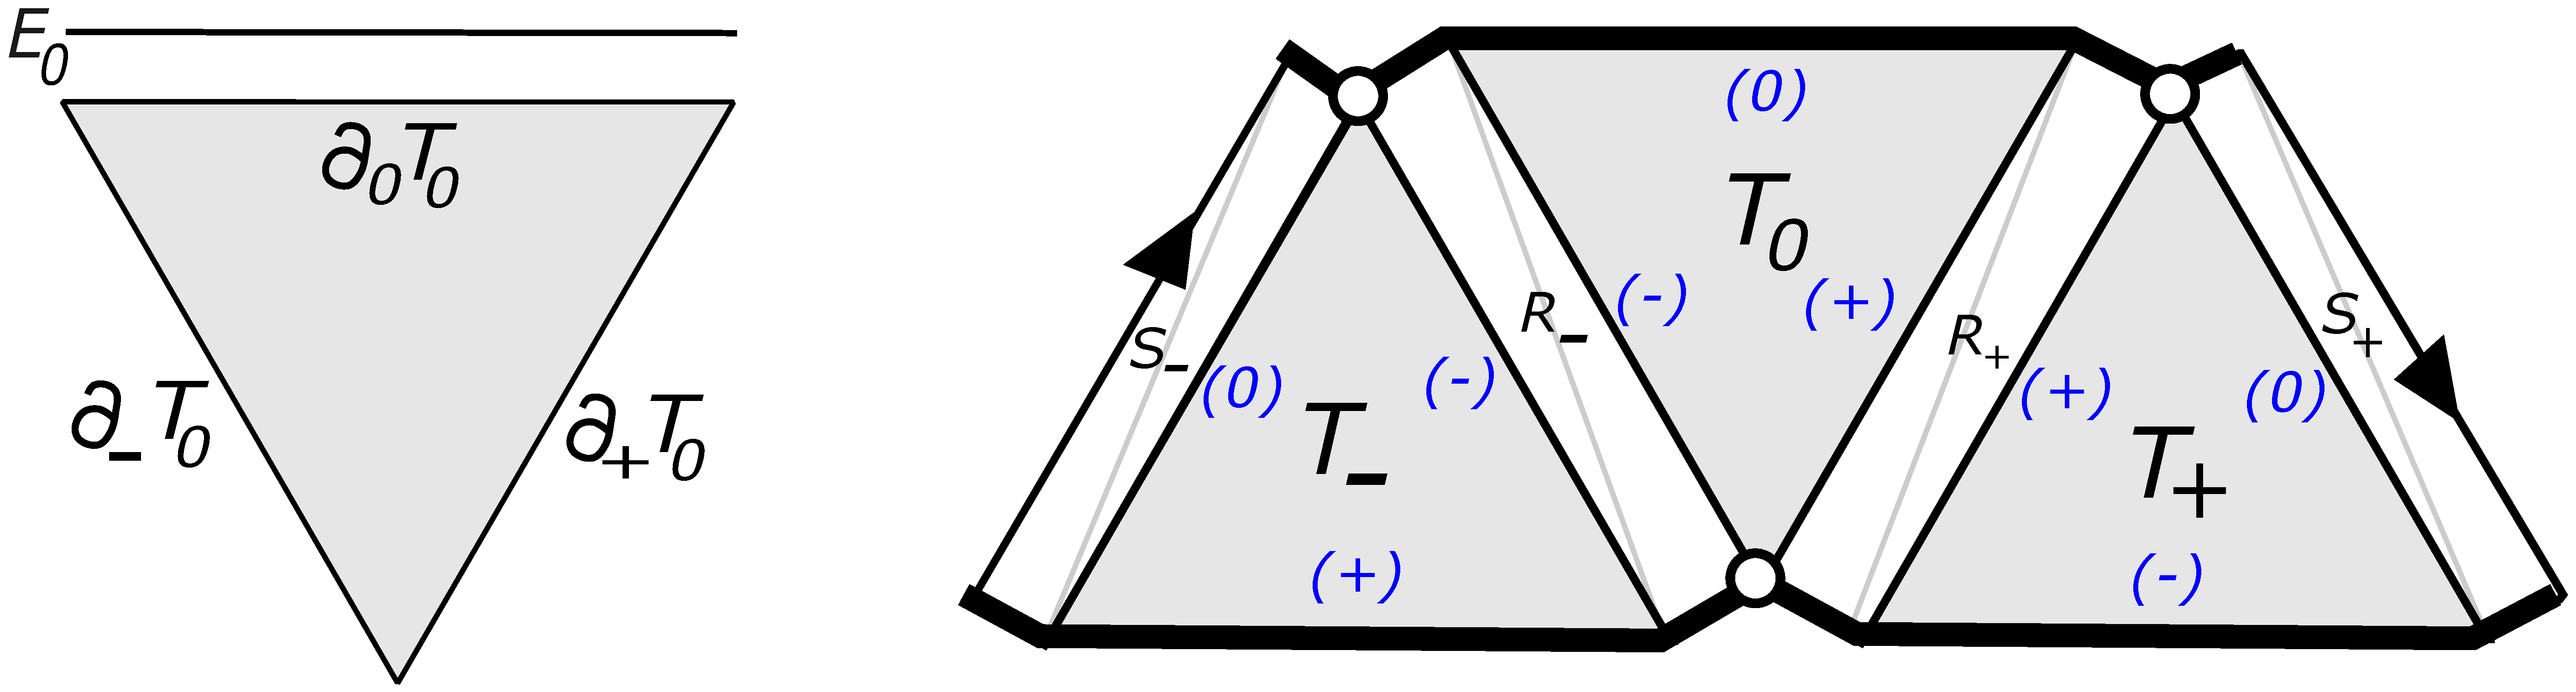
\includegraphics{fig2.eps}}
  \newline {\bf
    Figure 2:\/} Constructing the range.
\end{center}
  
  With the pieces
  ordered cyclically according to the listing in Equation \ref{OM},
  consecutive pieces intersect precisely along an edge of length
  $\mu+\epsilon^2$.  The remaining pairs of pieces are disjoint.
  Hence $\Omega$ is a piecewise affine surface
  with boundary.  Figure 2 (right) shows this, with the edge labels
  abbreviated.   To get from Figure 2 (right) to the true picture in
  $\R^3$, we fold $T_-$ under $T_0$ and
  we fold $T_+$ over $T_0$.  With the gluing diagram
  shown in Figure 2 (right), this folding makes the arrows line up
    in the same direction along $E_0$, as they should.
  So, the gluing pattern is correct.  Hence $\Omega$
  is a Moebius band (rather than a cylinder).

Finally,   we triangulate each of our $4$ rectangles by
  adding in a diagonal, as in Figure 2 (right).
  The long sides of the thin triangles all have length
  at least $\mu+\epsilon^2$ and the short sides have
  length less than $2\epsilon^3$.
  \newline
  \newline
  \noindent
  {\bf The Domain:\/}
  Call a clean triangle {\it wide\/} if it is isosceles and its
  distinguished side
  is longer than $\mu$.  The distinguished side of
  a wide clean triangle is longer than the other two sides.
  Hence there is a clean triangle $T_0'$ whose distinguished
  side has length in $(\mu+\epsilon^2,\mu+2\epsilon^2)$ and
  whose other sides have length less than $\mu+\epsilon^2$.
     We normalize so that the   distinguished
  edge of $T_0'$ lies in the top boundary component of $\Sigma$.
  Let $T'_{\pm}$ be clean and congruent triangles on either
  side of $T_0'$ such that the gap between $T_0'$ and
  $T_{\pm}'$ is a parallelogram $R_{\pm}'$ having short side length
  $2\epsilon^2$.   Let $S_{\pm}'$ denote the parallelograms
having short side length $\epsilon^2$ that lie on either
side of $T'_{\pm}$.  Figure 3 shows the union of these
three triangles and $4$ parallelograms.
    
\begin{center}
  \resizebox{!}{1.8in}{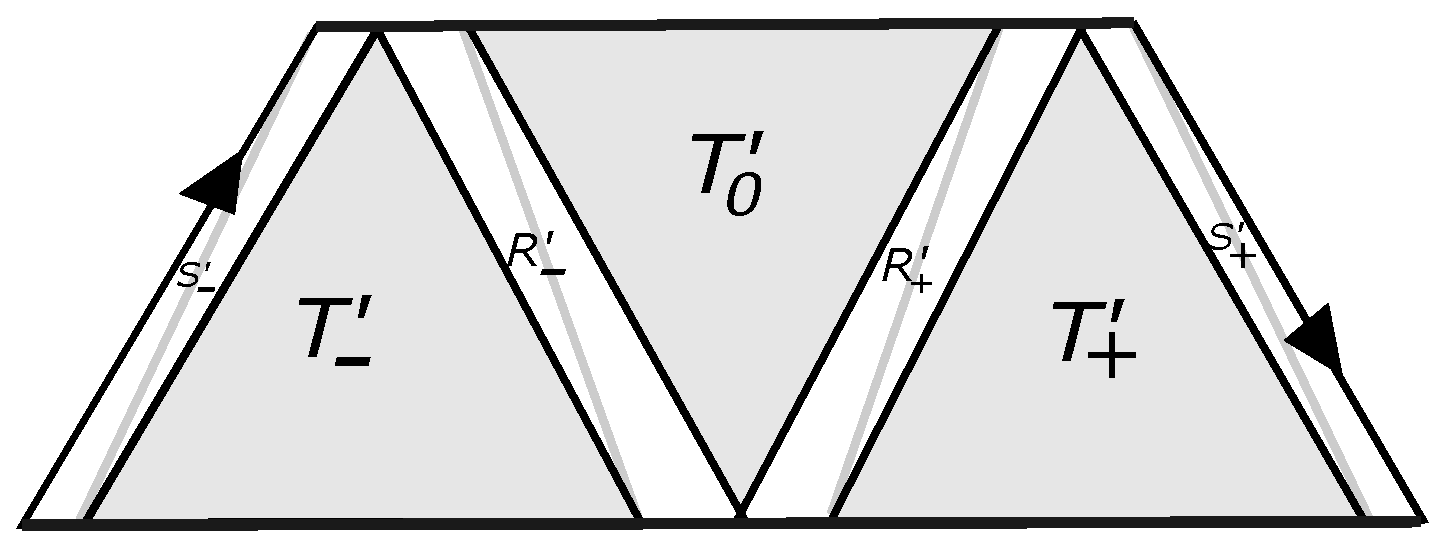
\includegraphics{fig4.eps}}
  \newline {\bf
    Figure 3:\/} The domain $\Omega'=\Sigma/G_{\beta}$ and
  its triangulation.
\end{center}

Note that $3\mu/2=\sqrt 3$.
Let $G_{\beta}$ be the glide reflection that identifies the
left side of $S'_-$ with the right side of $S'_+$.
The midline of $\Sigma$ intersects each of the three triangles
in Figure 3 in a segment of length at most $\mu/2+\epsilon^2$ and
two of the parallelograms in a segment of length $\epsilon^2$, and
two of the parallelograms in a segment of length $2\epsilon^2$.  Hence
$\beta<\sqrt 3+\epsilon$.
   The union of polygons in Figure 3 is a fundamental domain for the
   action of $G_{\beta}$ on $\Sigma$.
 The quotient $\Omega'=\Sigma/G_{\beta}$
 is a flat Moebius band.
\newline
\newline
{\bf The Map:\/}
As in Figure 3, we triangulate  the parallelograms in $\Omega'$ so as to always
use the short diagonals.  Each of these diagonals is shorter than
the long sides of the parallelograms.
Hence, each of these diagonals has length
less than $\mu+\epsilon^2$.   The triangulations
of $\Omega'$ and $\Omega$ are combinatorially identical and
hence determine an injective and continuous piecewise
affine map $\overline f$ from $\Omega'$ to $\Omega$.
 Let's check the squeeze condition.

\begin{itemize}
\item  On each $T_k'$, for $k \in \{0,+,-\}$,  the crosscutting edges
  have length less than $\mu + \epsilon^2$ and the
  distinguished edge has length greater than $\mu+\epsilon^2$.
  The map $\overline f$ carries all these edges to
  edges of length exactly $\mu+\epsilon^2$.  Hence
  $f$ has the squeeze property on $T_k'$.
\item On each thin triangle, the crosscutting edges (again)
  have length less than $\mu + \epsilon^2$ and the
  distinguished edges have length at least $\epsilon^2$.
  The map $\overline f$ carries the crosscutting edges to
  edges of length at least $\mu+\epsilon^2$ and the
  distinguished edges to edges of length
  at most $2\epsilon^3<\epsilon^2$.
  Hence $\overline f$ has the squeeze property on all
  thin triangles.
\end{itemize}

Therefore, the squeeze condition holds on every triangle.
Finally, we let $f: \Sigma \to \Omega$ be the equivalent lift of
$\overline f$.  More precisely, $f=\overline f \circ \pi$, where
$\pi: \Sigma \to \Omega'$ is the quotient map.
This map has all the required properties.
Hence $\beta<\sqrt 3 + \epsilon$ is realized.
This proves Statement 2.

   
  

\end{document}






 
